% !TeX root = ./main.tex
\documentclass{article}
\usepackage[utf8]{inputenc}
\usepackage{hyperref}
\usepackage{graphicx}
\usepackage{listings}

\title{CocosBCX - Traducción al español}
\author{Alexis Wolf Waisman }
\date{November 2019}

\begin{document}
\maketitle
\section{Comenzando}
\subsection{Introduction}
\subsubsection{¿Qué es Cocos-BCX?}
Cocos-BCX, la plataforma para la próxima generación de economía de juegos digitales, tiene como objetivo proporcionar a los desarrolladores de juegos una infraestructura de juegos de cadena de bloques fácil de usar y sólida, a la vez que ofrece a los usuarios un entorno de juego justo y abierto con datos transparentes y reglas claras. El mecanismo de consenso de la cadena de bloques subyacente está optimizado en base a la tecnología Graphene (grafeno). Con el sistema de contrato inteligente mejorado, Cocos-BCX es capaz de ofrecer un gran número de características para diversos juegos, tales como números aleatorios, sesión, temporizador y señales para verificación de calidad (HEARTHBEAT).
Esperamos ayudar a los desarrolladores y jugadores a asegurar un beneficio consistente a través del modelo económico de activos digitales soportados por la tecnología de cadenas de bloques:
\begin{itemize}
    \item Ayudar a los desarrolladores a asentar los contenidos que producen para obtener ganancias sostenibles a partir del uso, la gestión y la circulación de los activos de contenido proporcionando canales convenientes y descentralizados para la distribución de los juegos.
    \item Ayudar a los jugadores a convertir los datos generados por el tiempo y la energía que gastan, y los artículos obtenidos a través del consumo, en activos que puedan ser almacenados, gestionados y distribuidos de forma segura, otorgando a los jugadores los derechos para comercializarlos.
\end{itemize}

La Plataforma incluye:
\begin{enumerate}
    \item Un marco de desarrollo que soporta múltiples sistemas operativos y cadenas de bloqueo.
    \item Un IDE basado en datos para dApps que está totalmente programado y basado en componentes.
    \item Un sistema de cadena de bloques y componentes funcionales esenciales para aplicaciones de alto rendimiento mejorados sobre la base del marco de la tecnología Graphene (grafeno).
\end{enumerate}

Cocos-BCX habilita a los desarrolladores a programar, depurar y liberar dApps en conjunto con aplicaciones híbridas basadas en cadenas de bloques.
Además, la plataforma integra un sistema de libro mayor distribuido (DLS) basado en una cadena de bloques, un sistema de billetera criptográfica y una plataforma de circulación de activos digitales, permitiendo a los activos internos que los mismos se almacenen fuera de la cadena de forma permanente y se puedan utilizar en modo multi-cadena.
Teóricamente, el rendimiento de CocosChain TestNet puede alcanzar hasta 100.000 tps. Probamos 3.500 tps con intervalos de bloques de 3 segundos en un entorno experimental, es decir, se necesitan 3 segundos para que la información se transmita a toda la red.

El rendimiento mejorará aún más una vez que se haya completado el consenso definido en el contrato, el escalamiento multi-cadena y la delegación de testigos. Los algoritmos clave de la mayoría de los juegos pueden ser ejecutados en cadena, y la tecnología de "confirmación de transacciones con la latencia más baja" mejorará aún más la experiencia del proceso de circulación de activos.
La billetera basada en CocosChain TestNet puede integrarse en la plataforma de circulación de activos; en donde los usuarios pueden evaluar el valor de las monedas, objetos y cuentas del juego en función del tipo de cambio de los activos digitales del juego con respecto a la moneda base de la cadena principal.
Cocos-BCX está soportado por COCOS Creator, un editor de juegos, mediante el cual el juego desarrollado tradicionalmente puede ejecutarse en el entorno de tiempo de ejecución de la cadena de bloques Cocos-BCX.

\subsubsection{Características técnicas y funciones generales}
Cocos-BCX apunta a construir un entorno de ejecución completo para juegos multisistema, proporcionando a los desarrolladores de juegos bl la máxima comodidad y un ecosistema mejorado, a la vez que aporta a los jugadores una experiencia de juego totalmente nueva, así como formas de juego que son diferentes de las anteriores. Los usuarios disfrutarán de una autonomía considerable en la disposición de los activos del juego y de un entorno de juego justo y abierto.
Por lo tanto, Cocos-BCX está diseñado para ofrecer las siguientes características técnicas, que se describirán de manera enunciativa pero no taxativa:
\begin{enumerate}
    \item Un entorno de tiempo de ejecución de juego multiplataforma con interfaces interoperables de cadena de bloques.
    \item Un mecanismo de consenso mejorado basado en la prueba de la participación de los delegados (DPoS) y en la modalidad de testigos delegados.
    \item Una TestNet (red de pruebas) con transmisión de datos mejorada y una máquina virtual de alto rendimiento.
    \item Una pasarela de intercambio entre cadenas que admite activos digitales homogéneos y no homogéneos.
    \item BCX-NHAS-1808 estándar de activos digitales no homogéneos.
    \item Un sistema mejorado de permisos de los activos.
    \item Contratos inteligentes ejecutables entre bloques.
    \item Operación de transacción atómica (Todo-o-nada).
    \item Apoyo a las tareas de consenso a nivel sintáctico.
    \item Soporte para el mecanismo de transacciones delegadas.
    \item Consenso a pequeña escala y números aleatorios.
    \item Proceso aleatorio confiable en la cadena.
    \item Soporte para ciclos mínimos de validación de transacciones dentro de la cadena.
    \item Compatibilidad con contratos inteligentes para funciones clave del juego, como temporizador preciso, modo de espera y señalizador (heartbeat).
    \item Mecanismo de verificación de transacciones para evitar que BP/desarrollador haga trampas.
\end{enumerate}

Mientras tanto, Cocos-BCX proporciona funciones que incluyen, pero no se limitan a:
\begin{itemize}
    \item Interfaces inter-operables de activos sin intermediarios (props).
    \item Ejemplos de plataformas de circulación de activos no homogéneos.
    \item Autonomía del jugador y el mecanismo Smithy.
    \item IDE visualizado (programa del juego y edición visual del contrato).
    \item Cartera criptográfica completa, sistema de cuentas de usuario y explorador de bloques.
    \item Sistema iterativo de contratos inteligentes.
\end{itemize}

\subsubsection{Versiones}

\begin{table}[h!]
\centering
\begin{tabular}{||c   c ||} 
 \hline
 Componente & Versión \\
 \hline\hline
 witness\_node &   \\ 
 \hline
 cli\_wallet &   \\ 
 \hline
 JS SDK &   \\ 
 \hline\hline
\end{tabular}
\end{table}

\subsubsection{Requerimientos Técnicos}
\title{Programación LUA}\\
Dado el uso extensivo del lenguaje Lua en el desarrollo de juegos tradicionales y su accesibilidad, nuestra máquina virtual de contractual actualmente soporta Lua (Lua 5.3) y cubrirá además otros lenguajes como JavaScript, Solidity entre otros; Es fácil comenzar con Lua leyendo el Manual de Referencia de Lua 5.3: \url{https://www.lua.org/manual/5.3/}


\title{Desarrollo Front-End}\\
Las aplicaciones de la cadena de bloques pueden distinguirse de las tradicionales por las dos fórmulas siguientes:
\begin{itemize}
    \item\textbf{Aplicación = Frontend + Servidor} 
    \item\textbf{DApp = Frontend + Contratos} 
\end{itemize}
En los contratos proporcionados por Cocos-BCX de Lua, existen las siguientes 3 opciones para el front-end:
\begin{itemize}
    \item  Original Web JS\\
    Este es un método tradicional de desarrollo WEB, que consiste en llamar al SDK de JS proveído por Cocos-BCX para interactuar con el sistema Blockchain.
     \item  Nativo\\
    Esté se asimila al desarrollo en IOS y en Android que básicamente llama a la API nativa proveída por Cocos-BCX.
    \item  Creador\\
    Este modelo es familiar para los desarrolladores de videojuegos .Se ha integrado al IDE de Cocos-BCX el creador; este hace fácil el despliegue de aplicaciones multiplataforma.
\end{itemize}

\title{Líneas de comandos}
Las operaciones por líneas de Comandos son requeridas para el desarrollo de nodos y billeteras, por lo tanto, es muy recomendable tener conocimientos respectivos a los sistemas y consolas de Linux.    

\subsubsection{Entornos de desarrollo integrado}
\begin{itemize}
    \item Creator
    \item VSCode
    \item Sublime Text
    \item Atom 
\end{itemize}

\subsection{Instalación}
\subsubsection{Componentes}
\title{nodo Testigo}

programa nodo de la blockchain.

\title{billetera cliente}

Una billetera que soporta todas las instrucciones por líneas de comando cuya interacción se realiza con la blockchain. Los documentos técnicos específicos se encuentran en: \url{https://dev.cocosbcx.io/docs/22-cliwallet}

\subsubsection{Componentes}{Compilación de código fuente}
Aún por desarrollar

\subsubsection{Instalación desde los binarios}
\title{Ambiente Ubuntu}

\subsubsection{Instalación con Docker}
Aún por desarrollar

\subsection{Crear una cuenta}
\title\emph{Registro}\\
Te puedes registrar en la terminal de  Cocos-BCX en \url{http://cocos-terminal.com/}. Todavía hay mucho para mejorar en cuanto a "experiencia de usuario" de la terminal , a pesar de ello, esta equipada con un montón de características; incluidas las funciones del núcleo de billetera y el browser.\\

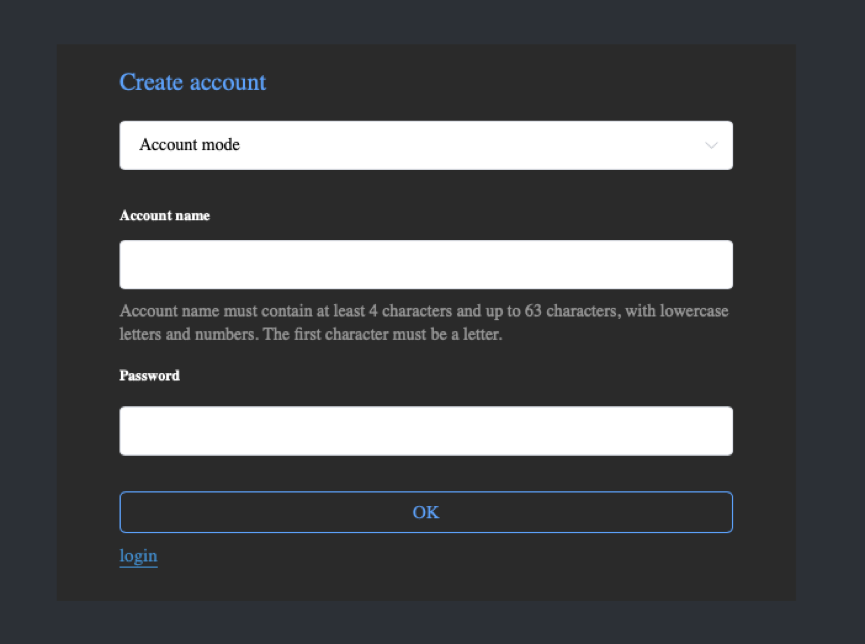
\includegraphics{Crate-an-account-1}\\


\title\emph{Ver claves privadas}\\
Para ver tus claves privadas debes hacer clic en "ver cuenta" dentro de la barra lateral, luego hacer clic en "copiar clave privada".

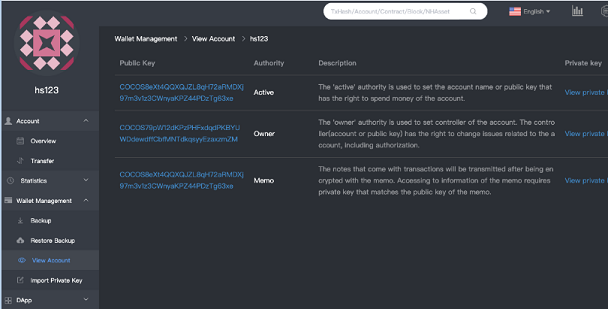
\includegraphics{Crate-an-account-2b}\\

\subsection{transferencia}
\title{autenticándose en la billetera por CLI}
\begin{enumerate}
    \item conseguir el ejecutable de líneaas de comando. (Archivo: cli\_wallet) y copiarlo en el directorio destino. 
    \item Dirigirse al directorio donde la billetera CLI fué alojada. Ejecutar los siguientes comandos para ingresar a la misma.\\
    \emph{comando: -chain-id [ID de cadena] [dirección del nodo RPC (testigo)] -r [ dirección desde la cual el servicio de RPC va a estar escuchando.]}
    \begin{lstlisting}[language=bash,caption={Autenticación}]
#!/bin/bash
./cli_wallet --chain-id 
81003974d328ff17b64076928ab87b24d7dffbc87df3d4cde89d2fa1877e4f6a -s 
ws://127.0.0.1:8070 -r 127.0.0.1:8099
# todo en una linea!!!!
    \end{lstlisting}
 \includegraphics{transfer-1}\\
    \end{enumerate}

\title{Configurar clave para la billetera}
\begin{enumerate}
    \item La primera vez que se realiza la autenticación  se debe establecer una contraseña.
    \emph{comando: set\_password}
    \begin{lstlisting}[language=bash,caption={Configurar password}]
     set_password xxxx
    \end{lstlisting}
     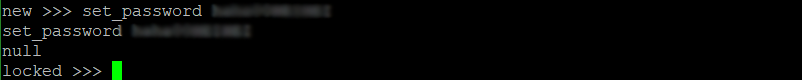
\includegraphics{transfer-2}\\
     \item Después de configurar la clave, se necesita desbloquear la billetera.
      \begin{lstlisting}[language=bash,caption={Configurar password}]
     unlock xxxx
    \end{lstlisting}
\end{enumerate}


 \title{Importar cuenta}
 \begin{enumerate}
    \item autenticarse en la billetera y ejecutar los siguientes comandos para importar la cuenta.\\
    \emph{comando: import\_key [nombre de usuario] [claves privadas de usuario]}\\
    \emph{clave privada: para ver la misma por favor remítase a la sección/subsección 1.3 de este mismo documento, en el apartado: \textbf{\textit{ver claves privadas}}]}\\
    \begin{lstlisting}[language=bash,caption={importar claves privadas}]
     import_key official-account 5KaVpJa9G4oqA5WHcSGitauFRuzdHcPVEAaESaA
    \end{lstlisting}
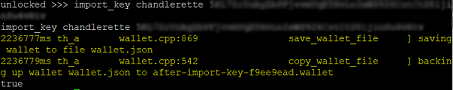
\includegraphics{transfer-3}
\end{enumerate}

\title{Importar los activos a la billetera}
\begin{enumerate}
    \item autenticarse en la billetera y ejecutar los siguientes comandos para importar la cuenta.\\
    \emph{comando: import\_balance [nombre de usuario] [clave privada correspondiente a la dirección del activo] [true/false]  }\\
    \emph{contexto: una nueva cadena cuyos activos iniciales no fueron exportados}\\
    \begin{lstlisting}[language=bash,caption={importar claves privadas}]
     import_balance official-account
     ["5KAUeN3Yv51FzpLGGf4S1ByKpMqVFNzXTJK7euqc3L"] true
    \end{lstlisting}
    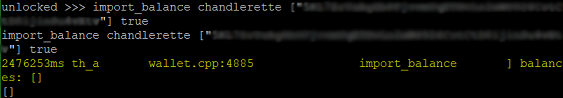
\includegraphics{transfer-4}
\end{enumerate}


\title{Importar los activos a la billetera}
\begin{enumerate}
    \item autenticarse en la billetera y ejecutar los siguientes comandos para importar la cuenta.\\
    \emph{comando: import\_balance [nombre de usuario] [clave privada correspondiente a la dirección del activo] [true/false]  }\\
    \emph{contexto: una nueva cadena cuyos activos iniciales no fueron exportados}\\
    \begin{lstlisting}[language=bash,caption={importar claves privadas}]
     import_balance official-account
     ["5KAUeN3Yv51FzpLGGf4S1ByKpMqVFNzXTJK7euqc3L"] true
    \end{lstlisting}
    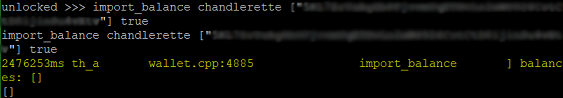
\includegraphics{transfer-4}
\end{enumerate}





\end{document}
